\section{Introdução}

% ----------------------------------------------------------------------------------------------------------
\begin{frame}{Contextualização}

Final de 2019, em Wuhan, China \cite{fagherazzi_2020}:
	
\begin{itemize}
	\item Casos de uma pneumonia não identificada reportados pela OMS;
	\item Variante do coronavírus, denominado \alert{SARS-CoV-2};
	\item \alert{Doença pelo Coronavírus 2019}, ou \alert{COVID-19};
\end{itemize}
	
O primeiro caso de COVID-19 no Brasil \cite{pinheiro_2020}:
\begin{itemize}
	\item  Hospital Albert Einstein, na cidade de São Paulo, em fevereiro de 2020.
\end{itemize}
	
\end{frame}
% ----------------------------------------------------------------------------------------------------------
\begin{frame}{Contextualização}

De acordo com o Worldometer \cite{worldometer_2021} em \sout{19 de abril de 2021} 07 junho de 2021:
\bigskip

\begin{columns}

\column{.40\textwidth}
      \begin{block}{\centering Casos Confirmados}
	      \centering
	      \bigskip
	      {\alert{\sout{13,9 Milhões}}}
	      \\ \smallskip
	      {\huge \alert{16,9 Milhões}}
	      \\ \smallskip
	        \textbf{3\textordmasculine\space Lugar Mundial}
	        
	        \bigskip
	\end{block}

\column{.40\textwidth}
      \begin{block}{\centering Óbitos Reportados}
	      \centering
	      \bigskip
	       {\alert{\sout{373 Mil}}}
	      \\ \smallskip
	      {\huge \alert{474 Mil}}
	      \\ \smallskip

	        \textbf{2\textordmasculine\space Lugar Mundial}
	        
	        \bigskip
	\end{block}

	
\end{columns}
\end{frame}

% ----------------------------------------------------------------------------------------------------------------------------------------------------------------------------------------------------
\begin{frame}{Contextualização}
	
\begin{columns}

\column{0.6\textwidth}
\begin{itemize}
	\item A pandemia da COVID-19 atingiu o país de maneira \alert{desigual} e com um alto grau de \alert{subnotificação de mortalidade} \cite{Veiga_JMIR_2020}; \bigskip
	\item Necessidade de analisar e definir as \alert{regiões de maior vulnerabilidade} \cite{campos2021vulnerability}; \bigskip
	\item Possibilitar o direcionamento de medidas de controle e contenção do vírus prioritariamente nessas regiões. \bigskip
\end{itemize}
		
\column{0.45\textwidth}
\begin{figure}[!h]  
%\caption{Evolução do número de óbitos por COVID-19 e SRAG nas regiões Brasileiras.}
	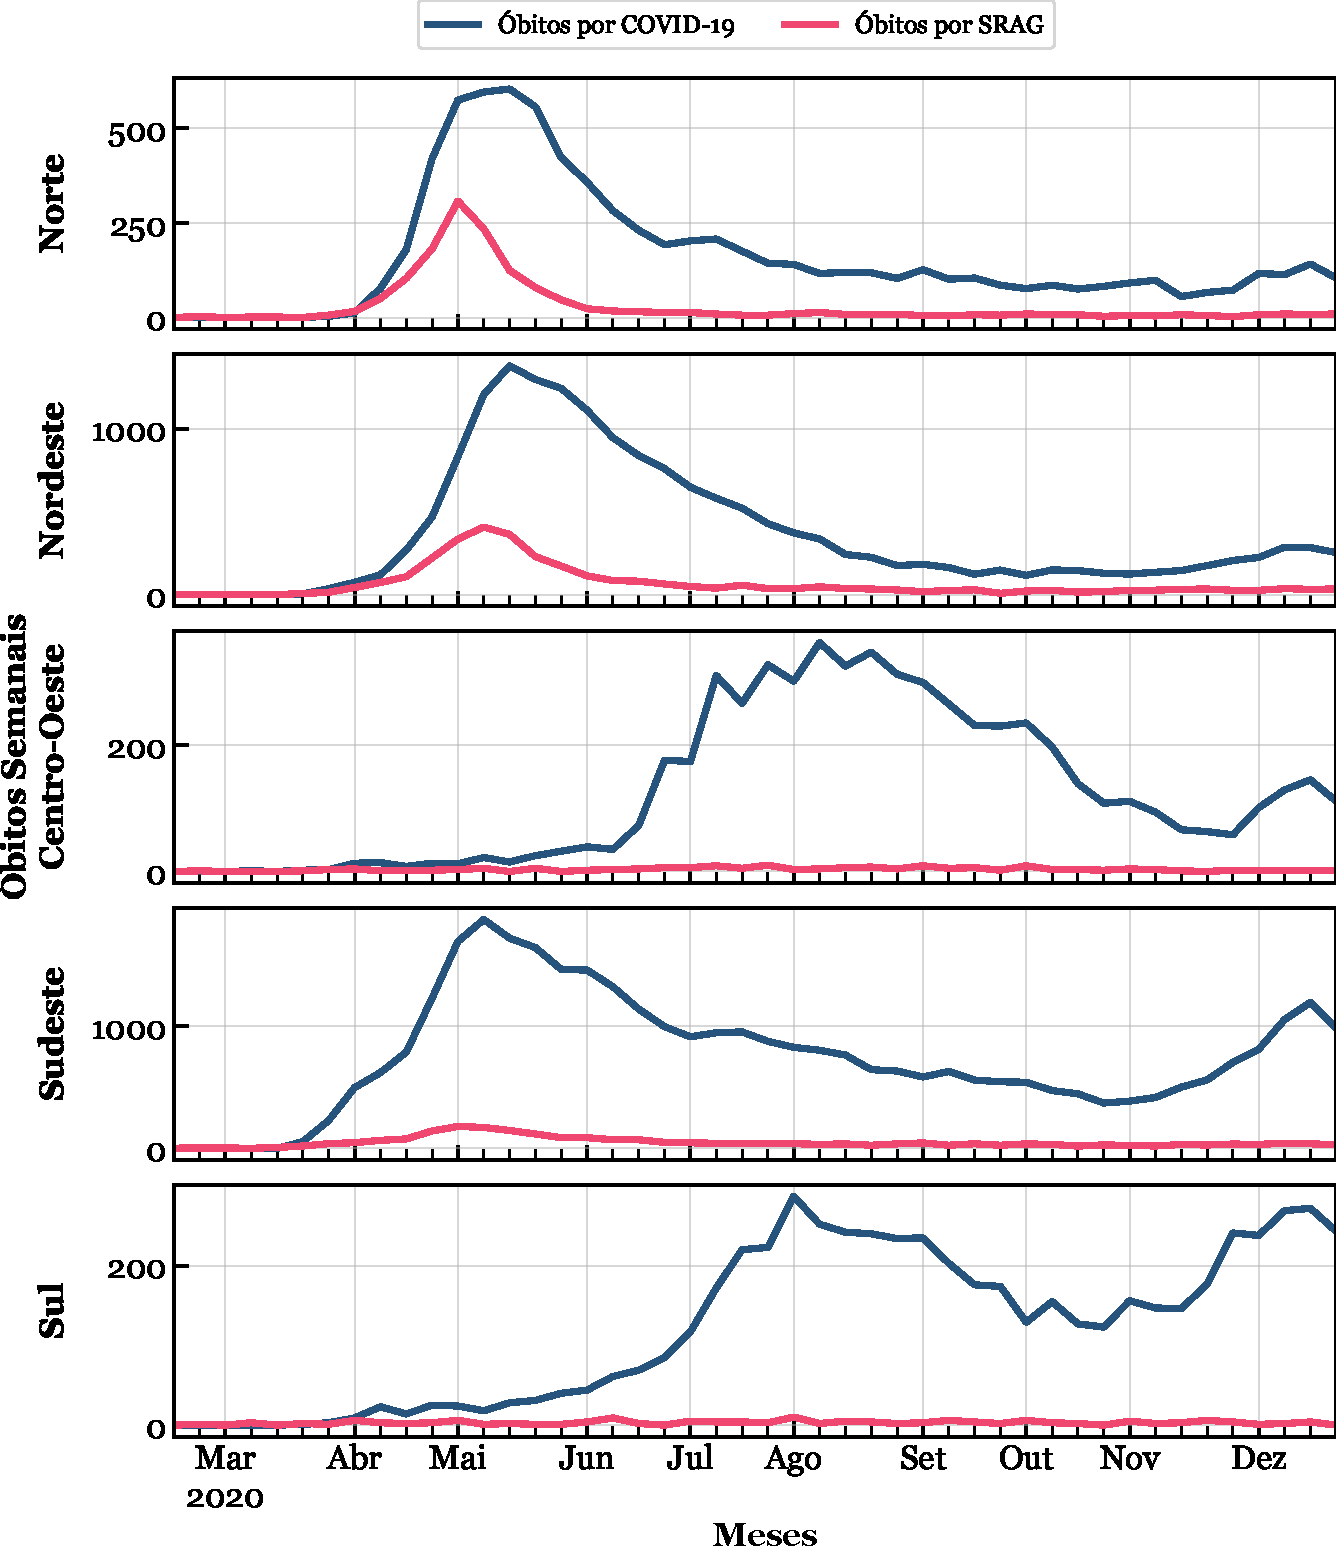
\includegraphics[width=\textwidth]{figs/obitos-regionais-2020}
%    \caption*{\footnotesize{Fonte: Elaborado pelo autor  (2021).}}
    \label{fig:regional-series-2020}
\end{figure}

\end{columns}

\end{frame}

% ----------------------------------------------------------------------------------------------------------------------------------------------------------------------------------------------------
\begin{frame}{Objetivo}

\begin{block}{Objetivo do Trabalho}
	\bigskip
	\Large Identificar as \alert{capitais brasileiras com maior vulnerabilidade} a pandemia do SARS-CoV-2, baseando-se em \alert{critérios sociais, econômicos, demográficos e epidemiológicos}.
	\bigskip
\end{block}

\end{frame}
